\documentclass[12pt]{article}
\usepackage[utf8]{inputenc}
\usepackage[T1]{fontenc}
\usepackage[french]{babel}
\usepackage{graphicx}
\usepackage{wrapfig}
\usepackage[includeheadfoot, top=0.65in, bottom=0.65in, left=1in, right=1in, headheight=12pt, headsep=0.55in]{geometry}
\usepackage{titlesec}


\setcounter{section}{-1}
\sloppy

\begin{document}

\begin{titlepage}
    \centering
    {\Huge Institut Informatique Appliquée\par}
    \vspace*{6cm}
    {\Huge \textbf{Rapport d'activité}}\par
    \vspace{.5cm}
    {\LARGE 2ème année de Manager en ingénieurie informatique}\par
    \vspace{0.4cm}
    {\Large Option Lead Dev}\par
    \vspace{9cm}
    {\Large Victor GIRAULT\par}
    \vspace{1cm}
    \vfill
    {\Large Année scolaire 2024 - 2025\par}
\end{titlepage}

\newpage
\tableofcontents
\thispagestyle{empty}
\newpage
\setcounter{page}{1}

\section{Introduction}
Ce mémoire a pour but de marquer l'aboutissement de mon parcours en master et représente une étape clé dans ma formation professionnelle. Il retrace le travail que j’ai effectué au sein de Niji, où j’ai eu l’opportunité de mettre en pratique les connaissances théoriques acquises au cours de mes études, tout en développant de nouvelles compétences dans un environnement professionnel exigeant. Cette année, j'ai évolué au sein du département DSF (Digital Software Factory) de l'antenne Rennaise de Niji, en tant qu'alternant "Ingénieur solutions".
\\\\
L’objectif de ce mémoire est de présenter de manière détaillée les missions qui m’ont été confiées, les méthodes et outils que j’ai utilisés, ainsi que les résultats obtenus. Il s’agit également de mettre en lumière les apprentissages tirés de cette expérience, tant sur le plan technique qu’humain, et de réfléchir à la manière dont cette immersion a enrichi ma compréhension des enjeux du secteur du développement informatique. Enfin, ce document vise à analyser les défis rencontrés et les solutions apportées, tout en proposant des pistes d’amélioration pour les projets futurs.
\\\\
À travers ce travail, je souhaite partager une vision à la fois critique et constructive de mon expérience en entreprise, en montrant comment elle a contribué à mon développement personnel et professionnel, et en soulignant son importance dans la construction de mon projet de carrière.
\\\\
J'ai intégré Niji en septembre 2024 en tant qu'alternant dans le cadre de ma deuxième année de formation de Manager en ingénieurie informatique (M2i) au sein de l'Institut Informatique Appliquée (IIA). À la suite de difficultés économiques et d'un manque de projets disponibles, j'ai été contraint de quitter l'entreprise d'alternance dans laquelle j'ai réalisé mes premières années en tant qu'alternant en développement informatique. Cette situation m'a poussé à rechercher une nouvelle entreprise pour poursuivre ma formation. Ayant réalisé mon année d'alternance de première année dans une petite entreprise de 4 employés, j'ai souhaité intégrer une entreprise de taille plus importante pour cette deuxième année afin de découvrir un environnement de travail différent et d'acquérir de nouvelles compétences. J'ai donc postulé chez Niji, une entreprise de services numériques (ESN) spécialisée dans le développement de solutions digitales.

\newpage
\section{Présentation de Niji}
\subsection{L'entreprise Niji}
\subsubsection{Historique}
\begin{figure}[h!]
    \centering
    \begin{minipage}{0.4\textwidth}
        \centering
        
\includegraphics[width=0.7\textwidth]{img/logo-niji.png} 
        \caption{Logo de l'entreprise Niji}
    \end{minipage}
    \hspace{0.05\textwidth}
    \begin{minipage}{0.4\textwidth}
        \centering
        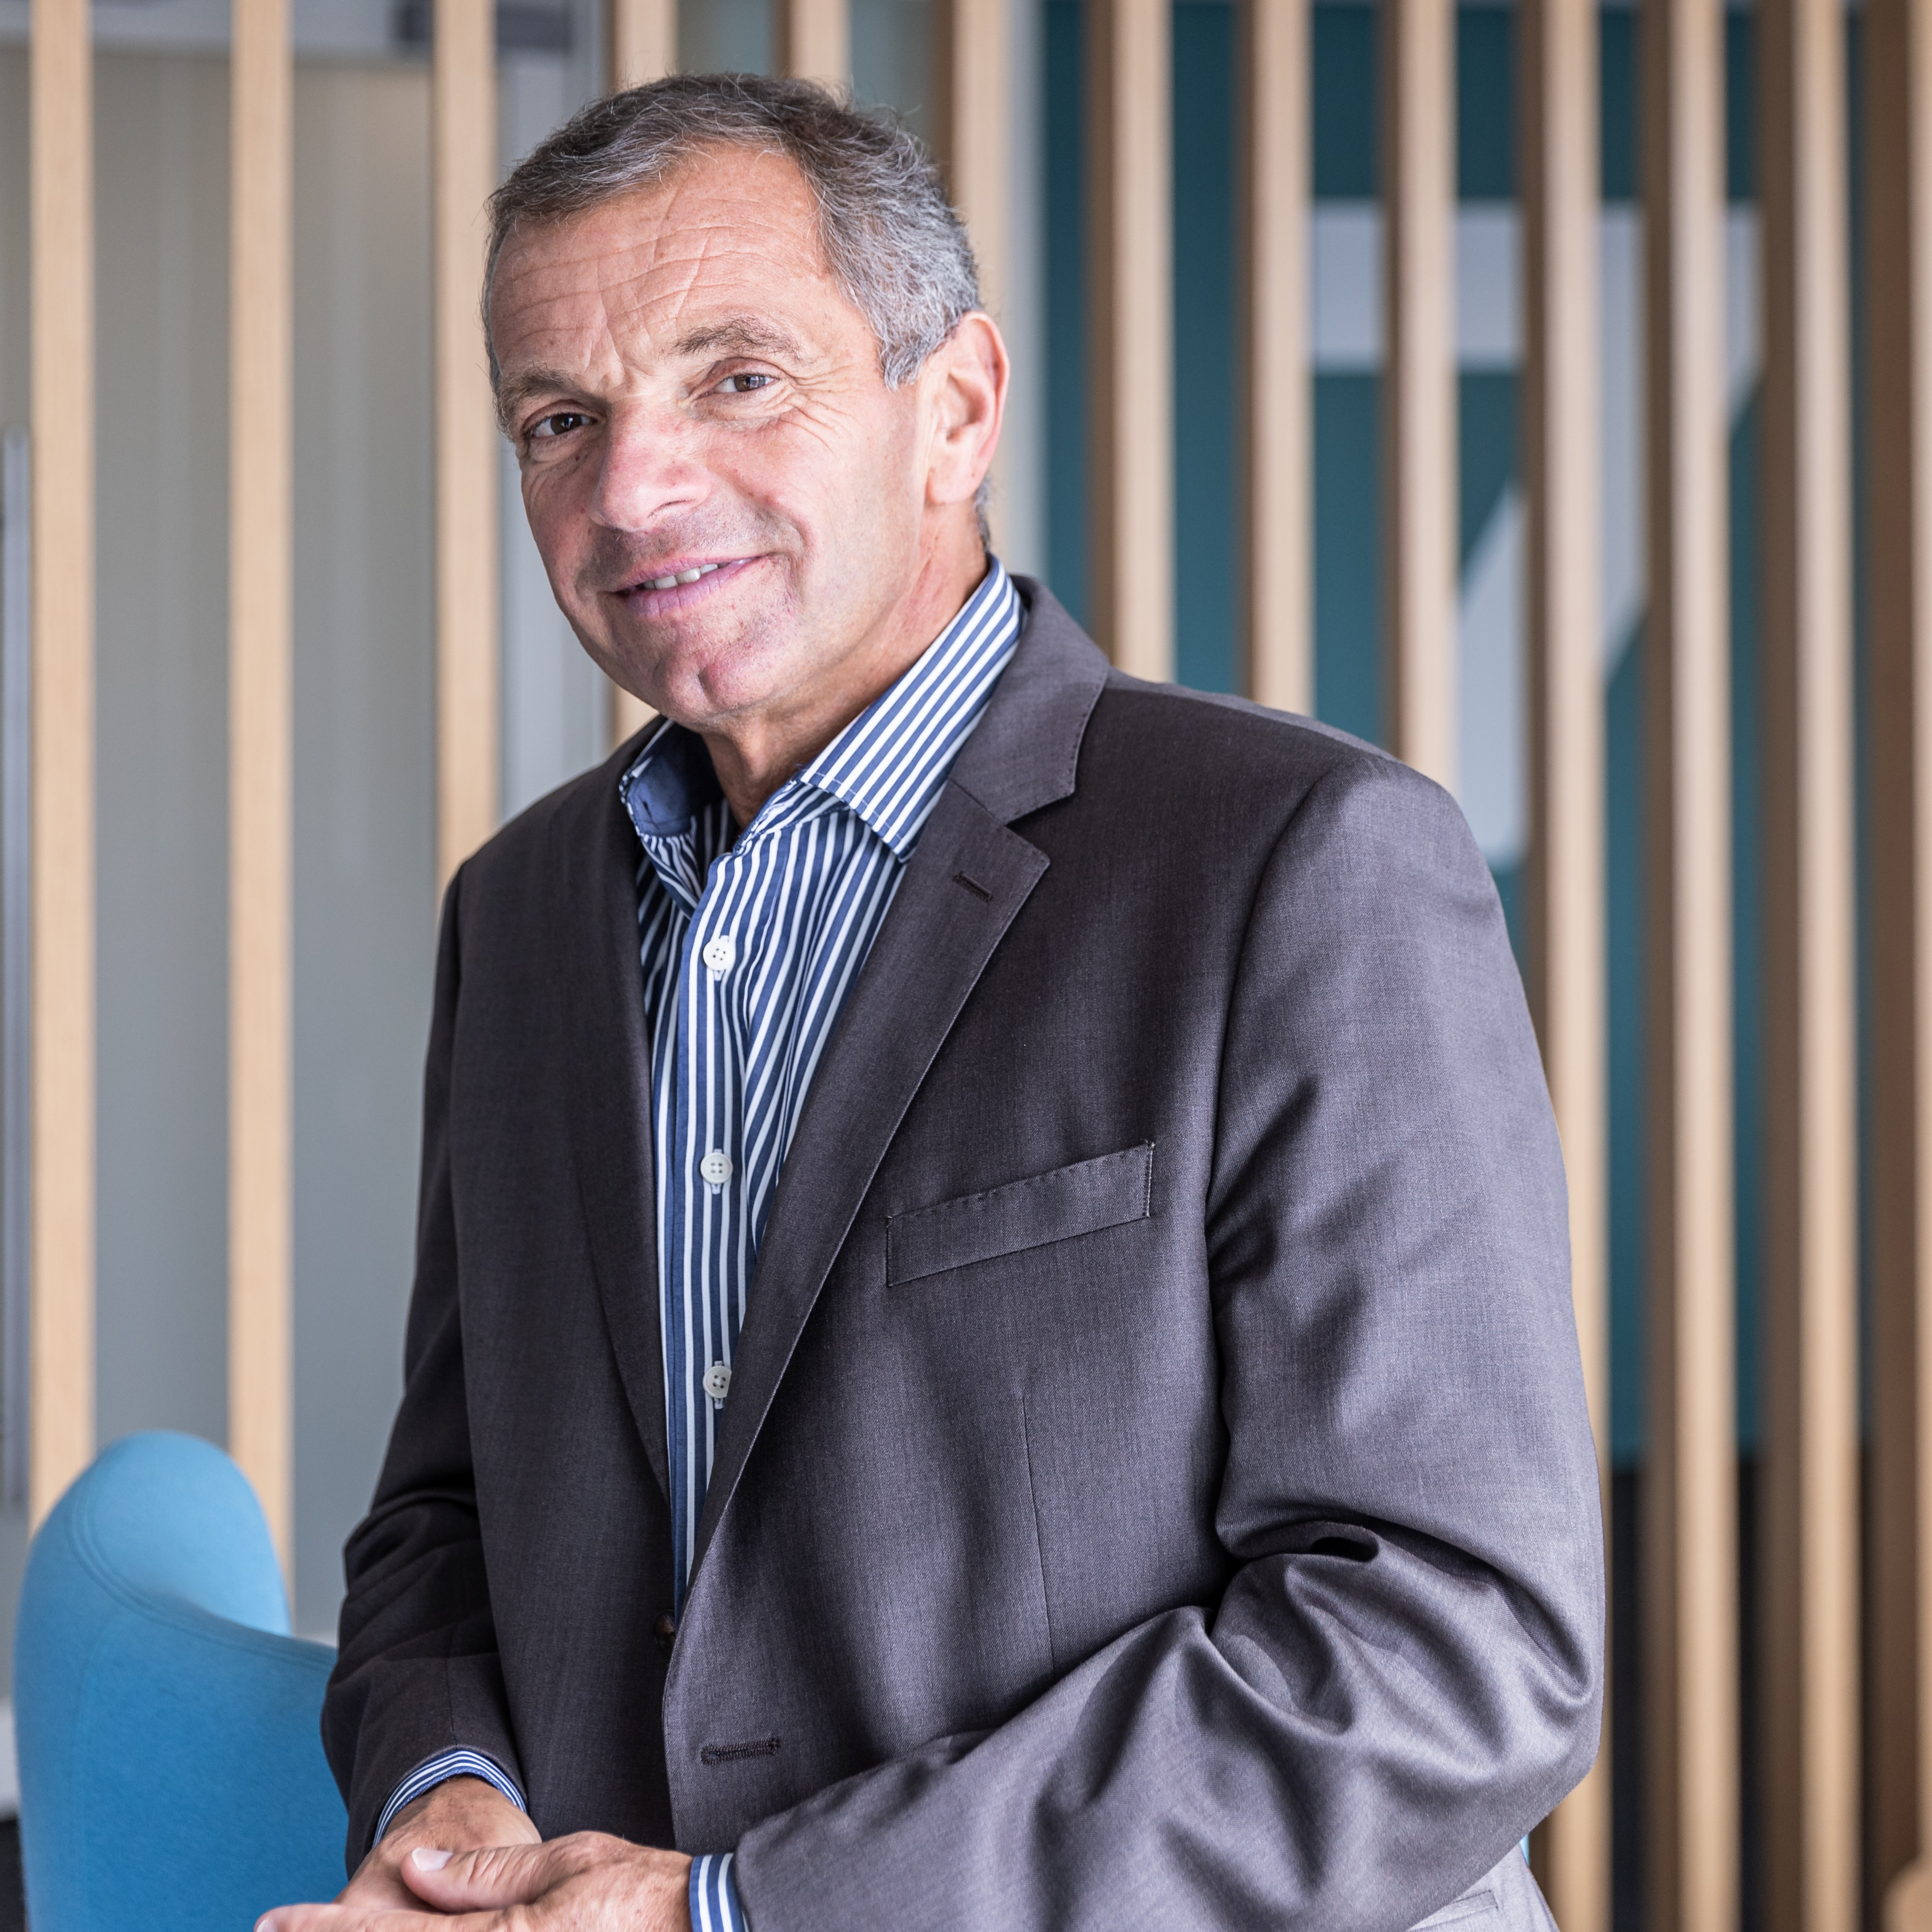
\includegraphics[width=0.7\textwidth]{img/hugues-meili.jpg}
        \caption{Hugues Meili}
    \end{minipage}
\end{figure}
Niji, qui signifie "arc-en-ciel" en japonais, est une entreprise co-fondée en septembre 2001 par Hugues Meili à Rennes. Niji est une ESN (Entreprise de service numérique) spécialisée dans le conseil, le design et le développement de solutions digitales pour des entreprises de toutes tailles. Depuis sa création, l'entreprise s'est imposée comme un acteur clé de la transformation numérique en France et à l'international.

\subsubsection{Les services proposés}
Niji se distingue par sa capacité à intervenir sur l'ensemble de la chaîne de valeur digitale. L'entreprise propose une large gamme de services adaptés aux besoins variés de ses clients. 
Tout d'abord, elle accompagne les entreprises dans la définition et la mise en œuvre de leur stratégie numérique. Cela inclut l'analyse des besoins métiers, l'identification des opportunités technologiques, et la conception de feuilles de route stratégiques alignées sur les objectifs de l'entreprise. Ce travail stratégique permet aux clients de mieux anticiper les évolutions du marché et de rester compétitifs.
\\\\
Ensuite, Niji excelle dans la conception de parcours utilisateurs innovants et intuitifs. Grâce à son expertise en design et en expérience utilisateur (UX/UI), l'entreprise crée des interfaces qui maximisent l'engagement des utilisateurs finaux. Cela inclut la réalisation de prototypes interactifs, des tests utilisateurs, et l'optimisation continue des interfaces pour garantir une expérience fluide et agréable.
\\\\
Enfin, Niji développe et déploie des solutions technologiques sur mesure, intégrant les dernières innovations du marché. Cela comprend le développement d'applications web et mobiles, la mise en place de plateformes cloud, l'intégration de systèmes complexes, et l'automatisation des processus métiers. L'entreprise s'appuie sur des méthodologies agiles pour garantir une livraison rapide et de haute qualité, tout en s'adaptant aux besoins évolutifs des clients.
\\\\
En complément, Niji propose également des services de maintenance et de support technique pour assurer la pérennité des solutions déployées. Cela inclut la gestion des incidents, les mises à jour régulières, et l'accompagnement des équipes internes des clients pour une prise en main optimale des outils développés.

\subsubsection{Les valeurs de l'entreprise}
Niji est une entreprise engagée dans la transformation numérique, qui accorde une grande importance à des valeurs humaines fortes.
\\\\
Loin d'être une simple formalité, la responsabilité sociétale des entreprises (RSE) est au cœur de la stratégie de Niji. Co-construite avec les collaborateurs, cette démarche s'articule autour de cinq axes : environnement, social, gouvernance, territoire et économie. Des actions concrètes sont mises en place pour réduire l'empreinte carbone, promouvoir l'égalité professionnelle, adopter une gouvernance éthique et soutenir le développement des territoires. Niji s'engage ainsi à contribuer au développement des entreprises, des talents et des territoires par un numérique utile.
\\\\
Chez Niji, la culture d'entreprise est profondément humaine. L'entreprise valorise le management de proximité, la transparence, la mobilité géographique et le bien-être au travail. Des initiatives telles que la plateforme de formation "Niji University", des événements internes réguliers et des activités sportives renforcent la cohésion et l'engagement des équipes. Cette approche favorise un environnement de travail motivant, challengeant et innovant.

\subsubsection{Les secteurs d'activité}
Niji intervient dans de nombreux secteurs d'activité, ce qui lui permet de diversifier ses expertises et de répondre à des besoins variés. Dans le domaine de la finance, elle développe des solutions pour les banques, les assurances et les fintechs. Elle accompagne également les opérateurs télécoms dans leur transformation numérique. Dans le secteur de l'énergie, Niji conçoit des solutions pour optimiser la gestion des ressources énergétiques. Elle contribue à la digitalisation des services publics pour améliorer l'expérience des citoyens et crée des parcours clients omnicanaux pour les enseignes de distribution.

\subsubsection{Les chiffres clés}
En 2025, Niji compte plus de 1300 collaborateurs répartis sur plusieurs sites en France et à l'international. L'entreprise, créée en 2001, réalise un chiffre d'affaires de 142 millions d'euros sur l'année 2024, avec une croissance de 20\% de son CA sur 5 ans, témoignant de sa solidité financière et de sa capacité à répondre aux attentes du marché. Elle est présente dans dix sites en France, notamment à Rennes, Paris, Lyon, Lille, Nantes, Angers, Bordeaux et Nice, ainsi que dans trois sites internationaux à Singapour et Casablanca. Encore récemment, Niji a ouvert un nouveau site à Madrid, en Espagne, suite au rachat de l'entreprise Neo9.

\subsubsection{Fonctionnement d'une ESN}
Une ESN (Entreprise de Services Numériques) est une entreprise spécialisée dans la fourniture de services informatiques et numériques. Elle intervient auprès de ses clients pour les accompagner dans leur transformation digitale, en proposant des solutions sur mesure adaptées à leurs besoins spécifiques. Le fonctionnement d'une ESN repose sur plusieurs éléments clés.
Tout d'abord, l'ESN recrute des experts dans divers domaines, tels que le développement logiciel, le design, la cybersécurité et le conseil. Ces experts sont ensuite affectés à des projets chez les clients, en fonction de leurs compétences et de leurs expériences. L'ESN agit en tant qu'intermédiaire entre ses collaborateurs et ses clients, en gérant les aspects administratifs, juridiques et financiers des missions.

\subsection{L'implantation géographique}
\subsubsection{Les sites en France}
Niji a commencé son aventure à Rennes, où se trouve toujours son siège social. Au fil des années, l'entreprise a ouvert des antennes dans plusieurs grandes villes françaises, notamment Paris, Lyon, Lille, Nantes, Angers, Bordeaux et Nice. Ces implantations permettent à Niji de rester proche de ses clients et de répondre rapidement à leurs besoins.

\subsubsection{L'expansion internationale}
Dans sa stratégie de croissance, Niji s'est également tournée vers l'international. L'ouverture de bureaux à Singapour, Casablanca et Madrid témoigne de sa volonté de conquérir de nouveaux marchés et de renforcer sa présence à l'étranger. Ces implantations permettent à Niji de collaborer avec des clients internationaux et de diversifier ses opportunités d'affaires.

\subsection{La culture d'entreprise}
\subsubsection{Le mode de travail}
Chez Niji, les collaborateurs bénéficient d'une grande flexibilité dans leur organisation. L'entreprise prône l'autonomie et la responsabilisation, tout en imposant des plages horaires communes pour favoriser les échanges. Le télétravail est également encouragé, avec deux jours par semaine proposés à l'ensemble des salariés. La plupart des collaborateurs travaillent en mode agile, ce qui leur permet de s'adapter rapidement aux besoins des clients et de livrer des projets de manière itérative. Cette approche favorise la collaboration, l'innovation et la réactivité, tout en garantissant une qualité de service optimale.
Un autre aspect important du mode de travail chez Niji est la collaboration à distance. En raison de la répartition des équipes sur différents sites en France et à l'international, ainsi que des projets menés avec des clients étrangers, les salariés travaillent très fréquemment en visioconférence. Cette organisation favorise les échanges entre collaborateurs de différents horizons et permet de maintenir une communication fluide, quel que soit le lieu de travail de chacun.

\subsubsection{La responsabilité sociétale}
Niji s'engage activement dans une démarche de responsabilité sociétale des entreprises (RSE). Cela se traduit par des actions concrètes en faveur du développement durable, de la diversité et de l'inclusion. L'entreprise soutient également des initiatives locales et encourage ses collaborateurs à s'impliquer dans des projets solidaires.
\\\\
Dans une démarche de développement durable, Niji s'efforce chaque année de réduire son empreinte carbone. L'entreprise met en place des actions concrètes pour limiter la production de CO2 liée à ses activités, que ce soit par l'optimisation des déplacements professionnels, la mise en place du télétravail, la sensibilisation des collaborateurs aux éco-gestes ou encore l'amélioration de l'efficacité énergétique de ses infrastructures. Cette volonté de diminuer progressivement la fabrication de CO2 s'inscrit dans la politique RSE de Niji et témoigne de son engagement en faveur de la transition écologique.

\subsection{Les perspectives d'avenir}
Niji ambitionne de poursuivre sa croissance en renforçant sa présence sur les marchés existants et en explorant de nouvelles opportunités.
Niji est en constante recherche de nouveaux talents pour accompagner sa croissance et répondre aux besoins variés de ses clients. L'entreprise recrute régulièrement des experts dans des domaines diversifiés, tels que le développement logiciel, la cybersécurité, le design UX/UI, ou encore l'intelligence artificielle. Cette stratégie de recrutement permet à Niji de rester à la pointe des innovations technologiques et d'offrir des solutions adaptées aux enjeux actuels.

\subsection{L'antenne Rennaise}
C'est en Bretagne, à Rennes, que Niji a ouvert sa première antenne en 2001. L'antenne Rennaise de Niji est aujourd'hui l'une des plus importantes de l'entreprise, avec plus de 300 collaborateurs. L'antenne Rennaise est un pôle d'excellence pour Niji, qui y développe des projets innovants et accompagne des clients de renom dans leur transformation digitale. Avec l'évolution de l'entreprise et les nouveaux bureaux ouverts dans les différentes villes de France, notamment à Paris, les bureaux bretons sont restés le siège social de l'entreprise notamment pour des raisons historiques mais surtout pour l'amour de la Bretagne du fondateur.
\\
Les bureaux de Niji à Rennes sont situés à EuroRennes, une nouvelle zone d'activité dynamique, à proximité de la gare et du centre-ville. S'étalant sur 3 étages, les locaux sont modernes et spacieux, offrant un cadre de travail agréable et stimulant pour les collaborateurs. Les bureaux Rennais sont équipés de salle de réunions, de cabines insonorisées, d'un espace de restauration avec une terrasse extérieure. Les espaces de travail sont modulables et permettent aux équipes de s'organiser selon leur besoins. 

\subsection{Imineti by Niji}
\begin{wrapfigure}{l}{0.32\textwidth}
    \centering
    
\includegraphics[width=0.75\linewidth]{img/imineti.jpg} 
    \caption{Logo de Imineti by Niji}
    \label{fig:wrapfig}
\end{wrapfigure}
Imineti by Niji est une branche de l'entreprise Niji spécialisée dans la gestion des risques numériques et la cybersécurité. Elle combine conseil en cybersécurité et expertise technique pour aider les entreprises à définir et mettre en œuvre des stratégies de sécurité efficaces. Imineti by Niji accompagne ses clients tout au long du processus, de l'analyse des risques et des tests d'intrusion jusqu'à la présentation des recommandations devant les comités de direction. L'objectif est de fournir une vision cohérente et à long terme de la sécurité, en aidant les entreprises à formaliser et à appliquer des règles de sécurité adaptées à leurs besoins.
\\
Imineti by Niji est localisé à Rennes, au sein de l'antenne Rennaise de Niji. Pour des raisons de sécurité et de confidentialité, l'accès aux bureaux d'Imineti est restreint. Si une personne non autorisée souhaite entrer dans les locaux d'Imineti, elle doit remplir une feuille en spécifiant son identité, son heure d'arrivée et de départ. Ainsi, les équipes d'Imineti peuvent savoir qui est présent dans les locaux à tout moment. De plus, l'accès aux bureaux d'Imineti est sécurisé par des badges magnétiques, ce qui permet de contrôler les entrées et sorties des personnes autorisées.

\subsection{Les différentes directions opérationelles de Niji}
À Niji, les collaborateurs sont répartis dans différentes directions opérationnelles. \\Ces directions opérationnelles sont :
\begin{itemize}
    \item DAF-SI : Direction Administrative, Financière et Systèmes d'information
    \item DRH : Direction des Ressources Humaines
    \item DCO : Direction Commerciale
    \item DCF : Digital Consulting Firm
    \item DDA : Digital Design Agency
    \item DSF : Digital Software Factory
    \item DST : Digital Smart Technologies
    \item DBS : Digital Business solutions
    \item DCS : Digital Cyber Security (Imineti by Niji)
    \item DDS : Digital Data solutions
\end{itemize}
\vspace{0.5cm}
Chaque direction opérationnelle est spécialisée dans un domaine particulier et travaille en étroite collaboration avec les autres directions pour offrir des solutions complètes et adaptées aux besoins des clients. Par exemple, la direction DCO (Direction Commerciale) est en charge de la prospection et de la relation client, tandis que la direction DDA (Digital Design Agency) se concentre sur le design et l'expérience utilisateur. La direction DCF (Digital Consulting Firm) est quant à elle spécialisée dans le conseil stratégique et l'accompagnement des clients dans leur transformation digitale.

\subsection{Le département DSF}
Durant mon contrat d'apprentissage avec Niji, j'ai intégré la direction opérationnelle DSF (Digital Software Factory). Ce département est en charge du développement des systèmes informatiques des clients de Niji.
\\\\
Le département est constitué de deux pôles principaux : le pôle "Build" et le pôle "Run". Le pôle "Build" est en charge de la conception et du développement de solutions digitales pour les clients de Niji, tandis que le pôle "Run" assure la maintenance et l'exploitation de projets déjà déployés et en production. Le pôle "Run" est également en charge de la gestion des incidents et des demandes de support technique.

\subsection{L'équipe avec laquelle j'ai travaillé}
Durant mon année d'alternance à Niji, je n'ai pas intégré d'équipe en particulier. En effet, j'ai été affecté à un projet interne de l'entreprise, qui n'était pas encore lancé. Aucune équipe n'a donc été formée pour ce projet. Cependant, j'ai eu l'occasion de travailler avec plusieurs collaborateurs de Niji :
\newline
\begin{itemize}
    \item Alban GREAU : Tuteur et responsable du projet NijiSkills
    \item Olivier DELALANDE : Développeur React
\end{itemize}
\paragraph{Alban GREAU} est le responsable du projet NijiSkills. Il a été mon tuteur durant mon année d'alternance et m'a accompagné tout au long de mon parcours chez Niji. Alban est architecte solution à Niji Rennes, et possède une solide expérience dans la gestion de projets digitaux. Il a su me guider et me conseiller dans mes missions, tout en me laissant une certaine autonomie pour développer mes compétences et donner mon avis sur certaines solutions.
\paragraph{Olivier DELALANDE} est un développeur React au sein de l'équipe DSF à Niji Paris. Il m'a rejoint sur le projet NijiSkills en tant que développeur en Avril 2025 afin d'apporter son expertise technique et de m'aider à développer le projet. Olivier a une forte expérience dans le développement d'application web avec React et a su me guider quant aux bonnes pratiques de développement. Il est intervenu notamment sur la partie de synchronisation des compétences entre l'application Nijskills et DoYouBuzz, une plateforme de création de CV en ligne.
\newpage
\section{Ma missions}
\subsection{Le projet NijiSkills}
Le projet sur lequel j'ai travaillé durant mon année d'alternance est un projet interne de l'entreprise Niji. Cette idée a été proposée par Alban Gréau et consiste en une application permettant de tracer les compétences de tous les collaborateurs de Niji. En outre, cette application offrirait également la possibilité de cocher les compétences d'un candidat lors d'un entretien, facilitant ainsi l'évaluation et le suivi des compétences au sein de l'entreprise.
\subsubsection{La naissance du projet}
Initié par Alban Gréau, le projet NijiSkills est né de la volonté de moderniser et d’optimiser la gestion des compétences au sein de l’entreprise. Constatant les limites des méthodes actuelles, principalement basées sur un tableau Excel peu structurant et difficile à exploiter pour comparer les candidats ou suivre les compétences, Alban a proposé de développer une application web dédiée. Celle-ci vise à centraliser les compétences des collaborateurs, à faciliter leur suivi dans le temps et à offrir une meilleure visualisation pour l’ensemble des parties prenantes. Ce projet s’inscrit dans une démarche globale de digitalisation et d’optimisation des processus internes de Niji, afin d’améliorer l’efficacité et la collaboration.
\\\\
Actuellement, les entretiens d’embauche s’appuient sur un tableau Excel conçu par Alban Gréau, qui contient des questions préformulées et permet de noter les réponses des candidats. Cette méthode montre toutefois ses limites, notamment pour comparer efficacement les profils ou partager les informations entre recruteurs, ce qui rend le processus moins fluide.

Par ailleurs, l’absence de vue centralisée sur les compétences des collaborateurs complique la recherche d’expertises en interne, que ce soit pour répondre à des besoins spécifiques ou constituer des équipes adaptées. NijiSkills a donc été imaginé pour répondre à ces enjeux et proposer une solution moderne, intuitive et collaborative.
\subsubsection{Les objectifs du projet}
Le projet NijiSkills a été conçu pour répondre à plusieurs besoins stratégiques identifiés au sein de Niji. Tout d'abord, il vise à améliorer les entretiens d'embauche en remplaçant le tableau Excel actuellement utilisé par Alban Gréau. Ce tableau, bien qu'utile, présente des limites en termes de structuration et de comparaison des candidats. L'application permettra de structurer les questions, de noter les réponses de manière standardisée et de faciliter la comparaison entre les candidats grâce à la visualisation des compétences sous forme de carte interactive.

Un autre objectif clé est de centraliser les compétences des collaborateurs dans une base de données unique et accessible. Cette centralisation permettra d'identifier rapidement les experts disponibles pour répondre à des besoins spécifiques, que ce soit pour des projets clients ou pour résoudre des problèmes internes. En outre, l'application offrira un moteur de recherche performant pour trouver les collaborateurs possédant des compétences précises.

Enfin, NijiSkills ambitionne de simplifier le suivi des compétences des collaborateurs. Les managers et les équipes RH pourront suivre l'évolution des compétences au fil du temps, identifier les besoins en formation et valoriser les parcours professionnels. Ce projet s'inscrit également dans une démarche de renforcement de la culture d'entreprise en valorisant les compétences et en favorisant une meilleure collaboration entre les équipes.


\subsubsection{Les fonctionnalités}
L'application NijiSkills propose plusieurs fonctionnalités essentielles. Elle offre une interface graphique intuitive permettant de naviguer dans une carte interactive des compétences, inspirée de l'application web Roadmap.sh. Cette carte permet de visualiser les compétences de manière claire et structurée.

En termes de gestion, l'application permet aux administrateurs d'ajouter, de modifier et de supprimer des compétences. Elle inclut également une fonctionnalité d'évaluation, qui permet aux managers de cocher les compétences d'un collaborateur ou d'un candidat lors d'un entretien. Cette fonctionnalité est particulièrement utile pour structurer les entretiens et faciliter la comparaison des profils.

Une autre fonctionnalité clé est la synchronisation avec la plateforme DoYouBuzz, qui permet d'importer automatiquement les compétences des CV des collaborateurs. Enfin, l'application propose des outils d'exportation de données pour générer des rapports ou des exports destinés aux besoins des RH ou des managers, ainsi qu'un moteur de recherche avancé pour trouver rapidement des collaborateurs possédant des compétences spécifiques.

\subsubsection{Les technologies utilisées}
Le projet NijiSkills a été développé en utilisant des technologies modernes et adaptées aux besoins du projet. Le framework Next.js a été choisi pour sa capacité à gérer des applications web performantes et optimisées, tout en offrant une excellente expérience utilisateur grâce à son rendu côté serveur (SSR) et son support des applications statiques. Ce choix a également permis de réaliser un "crash-test" pour évaluer les possibilités offertes par ce framework, qui n'était pas encore utilisé chez Niji.

Pour le design et le style de l'application, Tailwind CSS a été utilisé. Ce framework CSS utilitaire a permis de créer rapidement une interface utilisateur moderne et responsive, tout en garantissant une grande flexibilité dans la personnalisation des styles.

En ce qui concerne la gestion des données, l'ORM Prisma a été utilisé pour interagir avec une base de données PostgreSQL. Prisma a simplifié la gestion des requêtes et des migrations de base de données, tout en assurant une forte typage des données grâce à son intégration avec TypeScript. PostgreSQL, en tant que base de données relationnelle robuste et performante, a été choisie pour sa fiabilité et sa capacité à gérer des volumes importants de données.

\subsubsection{La méthodologie de développement}
Contrairement aux projets habituels menés par Niji, qui suivent une méthodologie Agile, le projet NijiSkills n'a pas suivi de méthodologie spécifique. En effet, le projet a été réalisé en grande partie par moi-même, sans équipe dédiée. Cependant, pour maintenir un minimum de suivi et d'organisation, l'outil Jira a été utilisé. Mon tuteur, Alban Gréau, y créait des tâches que je devais réaliser, ce qui permettait de structurer le travail et de suivre l'avancement du projet.

Cette approche, bien que moins formelle que les méthodologies Agile, a permis de garder une certaine visibilité sur le projet tout en s'adaptant à la nature individuelle de son développement. Cela m'a également permis de découvrir et de m'approprier des outils de gestion de projet utilisés chez Niji, tout en respectant les priorités définies par mon tuteur.

\subsection{Le développement de l'application}
\subsubsection{La création de l'application}
Le développement de l'application NijiSkills à débuté en septembre 2024, peu après mon arrivée chez Niji.
\subsubsection{L'architecture de l'applications}
\subsubsection{L'arrivée de Olivier DELALANDE sur le projet}
\subsubsection{La synchronisation des compétences avec DoYouBuzz}
\subsubsection{Mise en place d'un serveur MCP}


\end{document}